\documentclass[dvipsnames]{beamer}

\usepackage[utf8]{inputenc}
%\usepackage[dvipsnames]{xcolor}
\usepackage{pgfpages}
\usepackage{fancyvrb}
\usetheme{Madrid}

\definecolor{utorontoblue}{HTML}{00204e}
\colorlet{beamer@blendedblue}{utorontoblue}

\setbeamertemplate{navigation symbols}{}
% Uncomment line below for notes
% \setbeameroption{show notes on second screen}

\setbeamertemplate{note page}{\insertnote}


\title[Data Acquisition via APIs]{Data Acquisition via Application Programmable Interfaces}
\author{Adrian Petrescu}
\institute{Kinaxis}
\date{2021-11-04}

\begin{document}

\frame{\titlepage}


\begin{frame}
  \frametitle{Schedule}
  
  Part 1
  \begin{itemize}
    \item Introduction and motivation
    \item HTTP, REST, and the languages of the web
    \item Authentication schemes
    \item Lots and lots of practical examples
  \end{itemize}

  \alert{Part 2}
  \begin{itemize}
    \item Scraping unstructured data from the web
    \item Parsing 
    \item Automated spiders
  \end{itemize}

  Part 3
  \begin{itemize}
    \item The server-side of APIs
    \item Deploying to the Cloud
    \item Project Description
  \end{itemize}
\end{frame}


\begin{frame}
  \frametitle{Web Architecture}
  \framesubtitle{In Its Simplest Form}
  
\includegraphics[width=320pt]{img/web-architecture-1.png}
\end{frame}


\begin{frame}
  \frametitle{HTML \& CSS}
  \framesubtitle{Like Peanut Butter and Jelly}
  
\includegraphics[width=320pt]{img/html-css.png}
\end{frame}


\begin{frame}[fragile=singleslide]
  \frametitle{HTML}
  \framesubtitle{HyperText Markup Language}

  \begin{Verbatim}
    <HTML>
      <HEAD>
        <TITLE>Star Wars - Wikipedia</TITLE>
        <LINK REL="stylesheet" HREF="/static/style.css" />
      </HEAD>
      <BODY>
        ...
      </BODY>
    </HTML>
  \end{Verbatim}
\end{frame}


\begin{frame}[fragile=singleslide]
  \frametitle{HTML}
  \framesubtitle{HyperText Markup Language}

  \begin{block}{Links}
    \tiny
    \begin{Verbatim}
  <P>
    Never gonna <A HREF="https://www.youtube.com/watch?v=dQw4w9WgXcQ">give you up</A>
  </P>
    \end{Verbatim}
  \end{block}

  \begin{block}{Lists}
    \tiny
    \begin{Verbatim}
  <OL>
    <LI>Item 1</LI>
    <LI>Item 2</LI>
  </OL>
    \end{Verbatim}
  \end{block}

  \begin{block}{Images}
    \tiny
    \begin{Verbatim}
  <IMG SRC="https://www.google.com/images/branding/googlelogo/1x/googlelogo_color_272x92dp.png" />
    \end{Verbatim}
  \end{block}
\end{frame}


\begin{frame}[fragile=singleslide]
  \frametitle{HTML}
  \framesubtitle{HyperText Markup Language}

  \begin{block}{Tables}
    \tiny
    \begin{Verbatim}
  <table>
    <thead>
      <tr>
        <th>Month</th>
        <th>Savings</th>
      </tr>
    </thead>
    <tbody>
      <tr>
        <td>January</td>
        <td>$100</td>
      </tr>
      <tr>
        <td>February</td>
        <td>$80</td>
      </tr>
    </tbody>
    <tfoot>
      <tr>
        <td>Sum</td>
        <td>$180</td>
      </tr>
    </tfoot>
  </table>
		\end{Verbatim}
		\end{block}
\end{frame}


\begin{frame}[fragile=singleslide]
  \frametitle{HTML}
  \framesubtitle{HyperText Markup Language}

  \begin{block}{Div}
    \begin{Verbatim}
  <DIV ID="content" CLASS="full-width col">
    ...
  </DIV>
    \end{Verbatim}
  \end{block}

  \begin{block}{Span}
    \begin{Verbatim}
  <P>
    This November is the Wikipedia Donation Drive.
    <SPAN STYLE="color:#36c;">Come join us.</SPAN>
  </P>
    \end{Verbatim}
  \end{block}
\end{frame}


\begin{frame}[fragile=singleslide]
  \frametitle{CSS}
  \framesubtitle{Cascading Style Sheets}
 
  \begin{block}{Turn all links red}
    \begin{Verbatim}
  a {
    color: #ff0000;
  }
    \end{Verbatim}
  \end{block} 

  \begin{block}{Only use 80\% of the screen}
    \begin{Verbatim}
  body {
    width: 80%;
  }
    \end{Verbatim}
  \end{block}
\end{frame}


\begin{frame}[fragile=singleslide]
  \frametitle{CSS}
  \framesubtitle{Cascading Style Sheets}
 
  \begin{block}{Center-align tables in the sidebar}
    \begin{Verbatim}
  #sidebar table {
    text-align: center;
  }
    \end{Verbatim}
  \end{block} 

  \begin{block}{Color bookmarked headlines}
    \begin{Verbatim}
  h2.title.bookmarked {
    color: blue;
  }
    \end{Verbatim}
  \end{block}
\end{frame}


\begin{frame}[fragile=singleslide]
  \frametitle{CSS}
  \framesubtitle{Cascading Style Sheets}
 
  \begin{block}{Hide all non-HTTPS links in the sidebar}
    \begin{Verbatim}
  .sidebar :not(a[href^="https"]) {
    visibility: none;
  }
    \end{Verbatim}
  \end{block} 

  \begin{block}{Bold the first paragraph after any headline}
    \begin{Verbatim}
  h1,h2,h3+p {
    font-weight: bold;
  }
    \end{Verbatim}
  \end{block}
\end{frame}


\begin{frame}[fragile=singleslide]
  \frametitle{wget}

  \texttt{wget} is a very commonly-used utility for mirroring an entire URL hierarchy.
  It has very many flags, but a common starting point is:

  \bigskip

  \begin{block}{Common flags}
    \begin{Verbatim}
      $ wget -e robots=off -r -np [base-url]
    \end{Verbatim}
  \end{block}

  \bigskip

  As with any complex CLI tool, \texttt{man wget} is indispensable.
\end{frame}


\begin{frame}
  \frametitle{Breadth-First Traversal}
  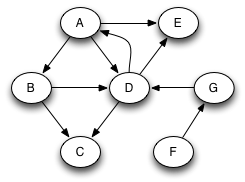
\includegraphics[width=320pt]{img/directed-cyclic-graph.png}
\end{frame}


\begin{frame}[fragile=singleslide]
  \frametitle{Breadth-First Traversal}
  \begin{block}{Algorithm}
    \begin{Verbatim}
def bft(g, root):
  seen = set()   
  q = [root]     
                 
  while q:       
    n = q.pop(0) 
    if n not in seen:
      visit(n)   
      seen.add(n)
      q += g[n]    
    \end{Verbatim}
  \end{block}
\end{frame}


\begin{frame}
  \frametitle{Web Architecture}
  \framesubtitle{In Its Modern Form}
  
\includegraphics[width=320pt]{img/web-architecture-2.png}
\end{frame}


\end{document}
